\item
Figure~\ref{fig:Disturbance_Observer_DO} shows the feedback interconnection for a system with a disturbance observer.
\begin{figure}[h]
    \centering
    \begin{minipage}{2.5in}
        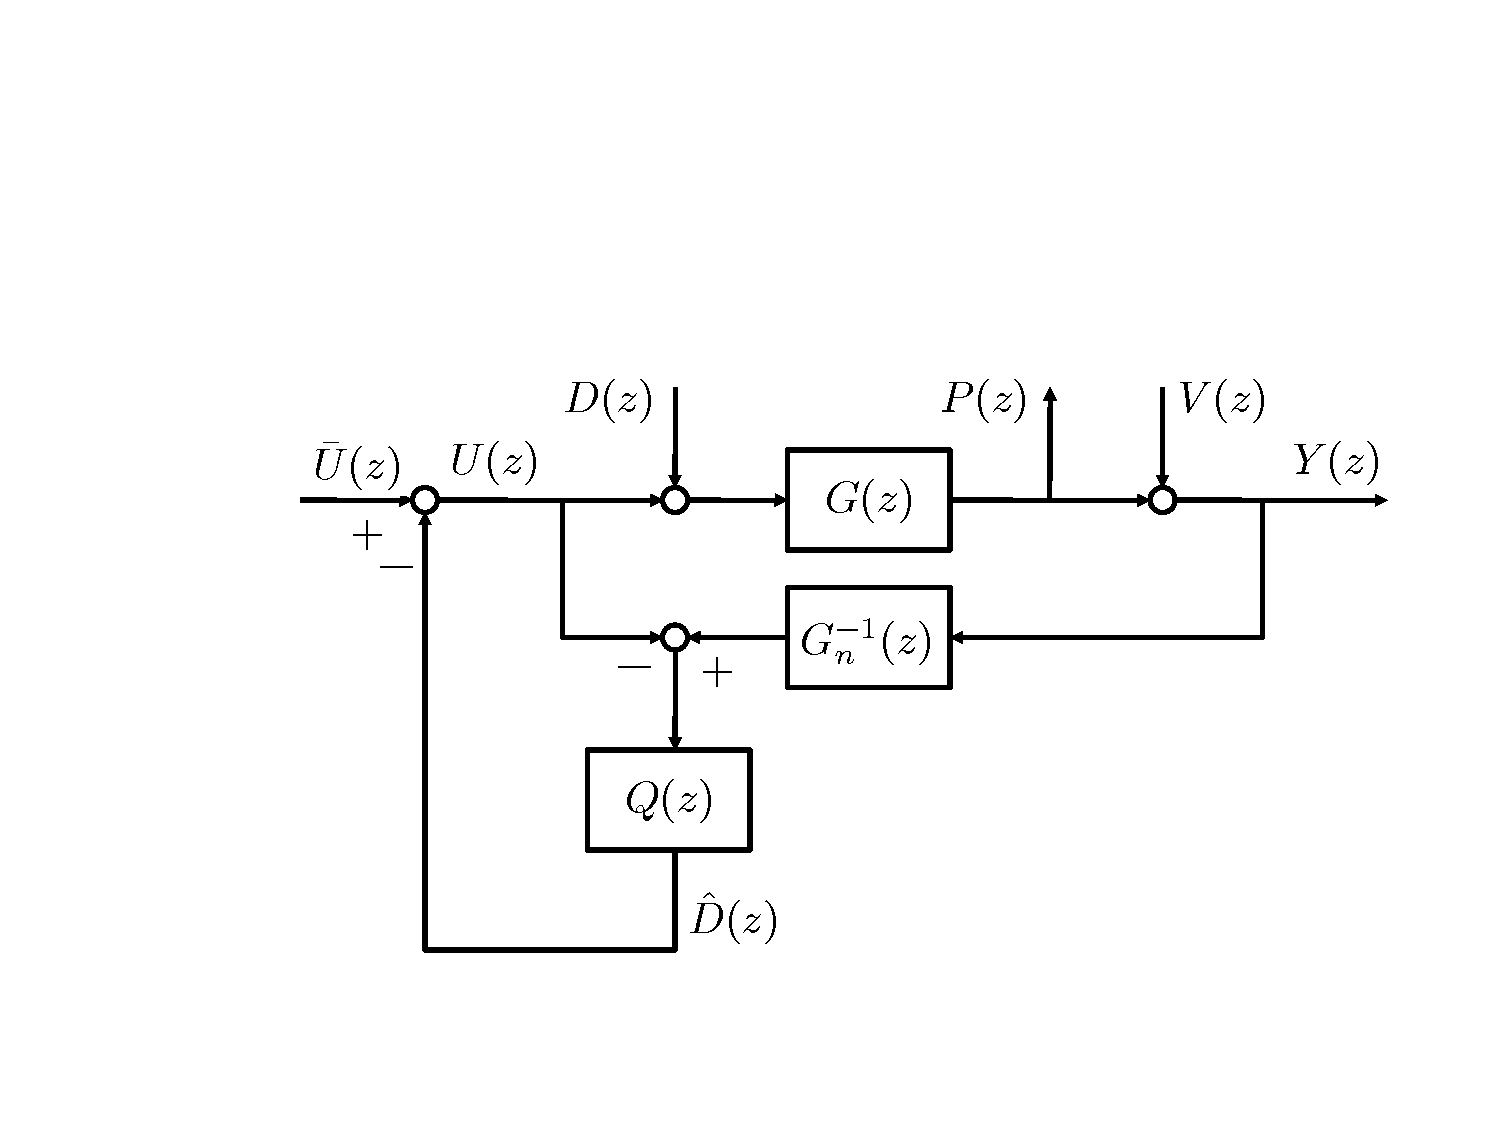
\includegraphics[width=2.5in]{Disturbance_Observer_DO}
        \caption{Disturbance Observer Structure}
        \label{fig:Disturbance_Observer_DO}
    \end{minipage}
    \qquad
    \begin{minipage}{2.5in}
        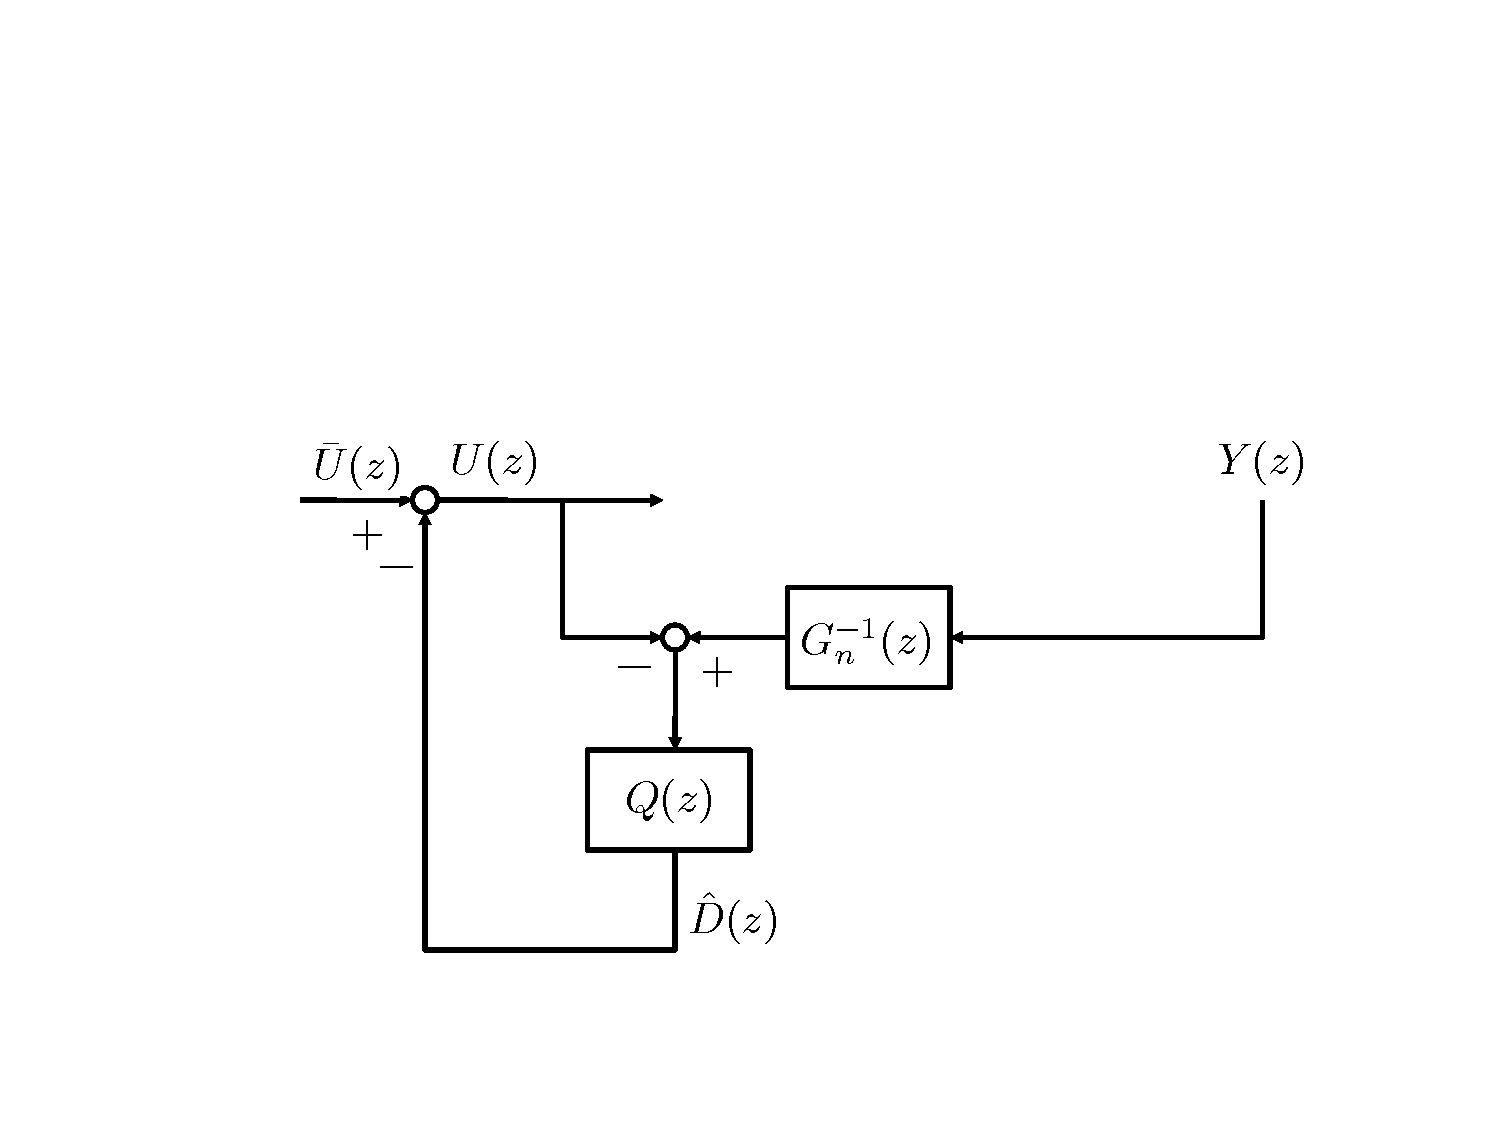
\includegraphics[width=2.5in]{Disturbance_Observer_controller}
        \caption{Disturbance Observer---Controller Only}
        \label{fig:Disturbance_Observer_controller}
    \end{minipage}
\end{figure}
When implementing the disturbance observer, we only implement the portion that generates $U(z)$ from $\bar{U}(z)$ and $Y(z)$, as shown in Fig.~\ref{fig:Disturbance_Observer_controller}.

\begin{enumerate}
    \item
    Find the transfer function from $Y(z)$ and $\bar{U}(z)$ to $U(z)$ in Fig.~\ref{fig:Disturbance_Observer_controller}.

    \item
    Suppose that $G_n^{-1}$ is proper. In this case, it is valid to choose $Q(z) = \alpha \in \mathcal{R}$. Based on your answer from the previous part, note that the block diagram in Fig.~\ref{fig:Disturbance_Observer_controller} is not well-posed when $\alpha = 1$. Does there exist $\alpha \in \mathcal{R}$ such that the closed-loop transfer function from $D(z)$ to $P(z)$ is zero? If not, is there a limit to how small we can make the transfer function from $D(z)$ to $P(z)$?

%    How should $\alpha$ be chosen when the primary control objective is disturbance rejection (i.e.\ if you neglect sensor noise and stability robustness)?
\end{enumerate}


